\section{Realisierung}
\subsection{Vorgehensweise}
Als Vorgehensweise wurde das erweiterte
Wasserfall-Modell gewählt. (Abbildung~\ref{fig:wasserfall_modell})
\begin{figure}[h]
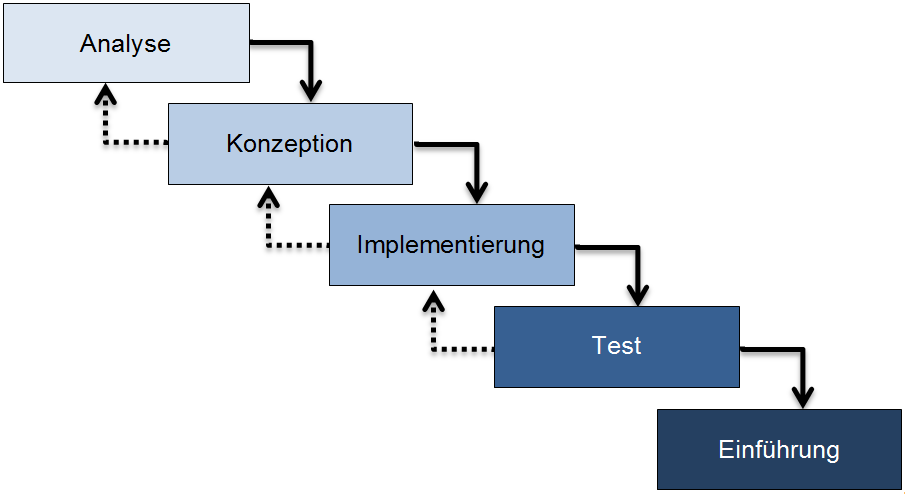
\includegraphics[scale=0.5]{img/wasserfall_modell.png}
\caption{Erweitertes Wasserfallmodell\label{fig:wasserfall_modell}}
\end{figure}
Aufgrund der knappen Zeitanforderungen bietet ein solcher Ansatz
den Vorteil eines direkten, klaren Pfades vom Beginn zum Ende des
Projektes. Im erweiterten Wasserfall-Modell erhält man, durch die
Möglichkeit kleine Rückschritte zu machen, die nötige Flexibilität um
auf Feedback einzugehen und Dinge ausprobieren zu können.
\subsection{Analyse \& Konzeption}
Bei der Analyse der Anforderungen fallen die Realtime Aspekte auf. Sie
sollen mithilfe von Websocketkommunikation und Push-Based-Updates vom
Server umgesetzt werden. Für einen modernen Look und ein intuitives
Verhalten soll die Steuerung Drag and Drop unterstützen.
\subsubsection{Architektur}
Zu Beginn wurde ein Plan für das grobe Zusammenspiel der beteiligten
Komponenten angefertigt. Hiermit wurde die Arbeit in mehrere Schritte
und leicht abzugrenzende Komponenten unterteilt. Das Projekt ließ sich
damit in Meilensteine aufteilen, um strukturiert an das Projekt
herangehen zu können.

Die Architektur gibt dabei folgende Aufteilung her:
\begin{itemize}
\item Datenbank
\item Backend Server
\item Desktop Frontend
\item Mobile Frontend
\end{itemize}
Einen Überblick über die spätere ``physikalische Ausprägung'' des
Systems soll Abbildung~\ref{fig:architektur} geben.
\begin{figure}[h]
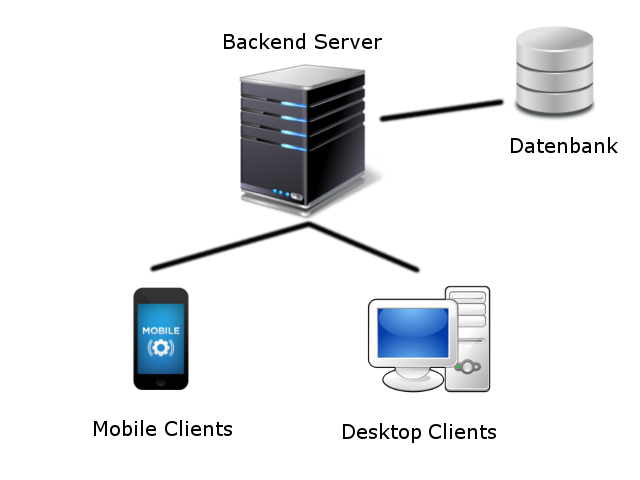
\includegraphics[scale=0.5]{img/Architektur.png}
\caption{Architektur Übersicht\label{fig:architektur}}
\end{figure}
Die Clients (Mobile / Desktop) kommunizieren über WebSockets mit dem
Backend-Server. Dieser speichert und liest Daten aus einer Datenbank.
Durch die WebSockets ist es dem Backend-Server möglich Änderungen am
Datenmodell mittels Push-Benachrichtigungen an die Clients weiterzugeben.
\subsection{Implementierung}
\subsubsection{Browser-Frontend}
Die Implementierung des Browser-Frontends verwendet Technologien, die
dem \gls{Reactive Programming} Pattern zuzuweisen sind. \gls{React} als
UI-Framework von Facebook ist ein stark durch funktionale Ideen und
\gls{Reactive Programming} inspiriertes Framework. Das Browser
Frontend ist modular aufgebaut, wobei das Modulsystem von
\gls{PureScript} behilflich ist. Ein Modul kapselt dabei die Definitionen innerhalb
einer Datei und kann von anderen Modulen importiert werden. Die
Kommunikation mittels WebSockets und das Verwalten des
Applikationszustandes geschieht in der in \gls{PureScript} implementierten
Engine. Dieser Teil des Programmes nimmt im Unidirectional-Dataflow
Modell die Rolle der ``Stores'' ein und erlaubt es das View-Layer
beliebig auszutauschen. Die Engine ist für alle Clients gleich und
kann daher für die mobile Version des Clients wiederverwendet werden.
\begin{figure}[h]
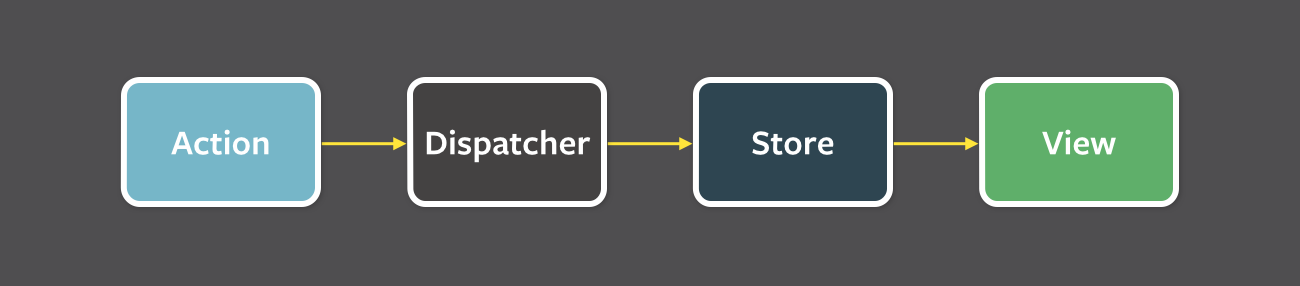
\includegraphics[scale=0.3]{img/Unidirectional.png}
\caption{Unidirectional Dataflow}
\end{figure}

\noindent Die Engine ``pusht'' den Applikationszustand in das
View-Layer, welches aus diesem ein User Interface rendert.
Die Interaktionen des Benutzers mit dem View-Layer erzeugen dann
wiederum Events, die als Streams an die Engine zurückfließen, wo sie
interpretiert und verarbeitet werden. Das Interpretieren der Events
lässt sich, dank des deklarativen Stils den PureScript erlaubt, leicht
programmieren. Als Beispiel soll der Code dienen, der das Ziehen eines
Themas auf das Grid beschreibt.

\begin{lstlisting}
  dragTopic = do
    Right t <- dragStart
    action <- dragOver
    lookup "dragEndTopic" `merge` lookup "dragEndGridTopic"
    return $ action t
\end{lstlisting}
\noindent Hier werden die Eventstreams für den Beginn eines
Drag Vorgangs sowie das Ziehen über einen Zeitslot mit dem Beenden des
Drag Vorgangs kombiniert und in einem resultierenden Stream \texttt{dragTopic}
ausgegeben. Dieser Stream abstrahiert nun die Mechanik des Drag and
Drop Vorganges und erlaubt es die tatsächlichen Intentionen des
Nutzers zu modellieren, um angemessen auf diese reagieren zu können.
\subsubsection{Backend Server}
Für die Entwicklung des Backend Servers wurde Haskell als
Programmiersprache ausgewählt. Haskell ist eine rein funktionale
Sprache und bringt dadurch die schon angesprochenen Vorteil im Bezug
auf Modularität und Skalierbarkeit mit sich. Die Implementierung
verwendet das \gls{Yesod Framework}, welches bereits Funktion für das
Ausliefern von HTML, CSS und JavaScript bereitstellt. Weiterhin erleichtert
das \texttt{Yesod.WebSockets} Modul das Programmieren der WebSocket Endpunkte.
\subsection{Test \& Abnahme}
Der Client wurde auf verschiedenen Endgeräten getestet. Hierbei fielen
immer wieder Kleinigkeiten auf, die sich unterschieden. Das Beheben
dieser kleinen Bugs gestaltete sich als zu zeitaufwendig, und so wurden
die unterstützten Browser auf Firefox und Chrome festgelegt.
Die Mobile Version wurde sowohl auf Android als auch auf iOS ausgiebig
getestet und funktioniert ohne Einschränkungen auf beiden Systemen.

%%% Local Variables:
%%% mode: latex
%%% TeX-master: "../Doku"
%%% End:
